\chapter{Medical and Technical Concepts}

\section{Introduction}
This chapter provides essential background information on the clinical and technological context of the thesis. We begin by describing the brain and its tissues from both macroscopic and microscopic perspectives. We then discuss brain tumors, which are the primary focus of this research. Next, we introduce the different types of medical imaging modalities and explain the importance of segmentation tasks in neuro-oncology. Finally, we delve deeper into the principles and components of Magnetic Resonance Imaging (MRI), which is the primary imaging modality used in this thesis.

\section{Macroscopic and Microscopic Description of the Brain}

\subsection{Macroscopic Description}
The human brain is an irregular, ovoid organ with a large anteroposterior axis. Its average volume is approximately 1100\,cm\textsuperscript{3} in women and 1400\,cm\textsuperscript{3} in men, and it weighs between 1400\,g and 1800\,g. It occupies the cranial cavity but does not contact the bone directly, as it is suspended in cerebrospinal fluid inside a fluid chamber \cite{ref3}.

The brain comprises four main regions: the cerebrum, cerebellum, brainstem, and diencephalon (Figure~\ref{fig:brain-regions}).

\begin{figure}[ht]
  \centering
  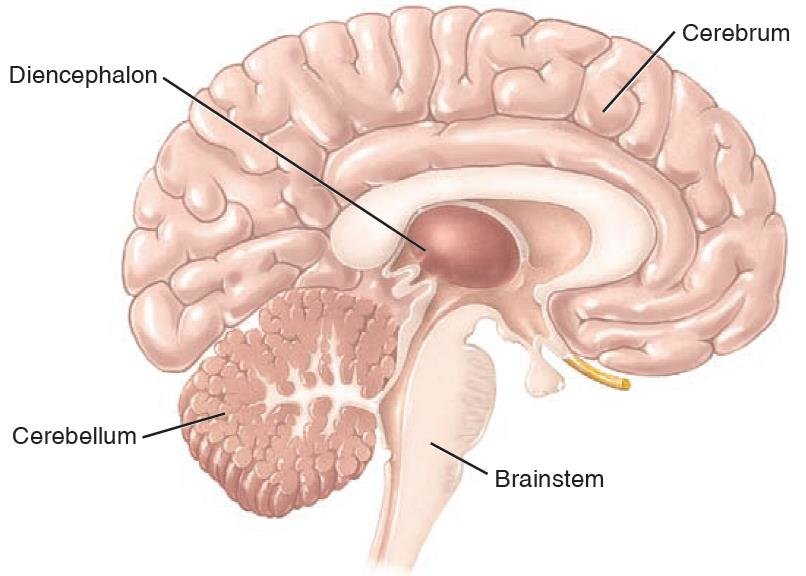
\includegraphics[width=0.5\textwidth]{Images/Chapter0/brain.jpg}
  \caption{Brain main parts: cerebrum, cerebellum, brainstem, and diencephalon \cite{freudenrich2013visualizing}.}
  \label{fig:brain-regions}
\end{figure}

\subsubsection{Cerebrum}
The cerebrum is the largest part of the brain, representing about 83\% of its total volume. It is divided into right and left hemispheres connected by the corpus callosum. Each hemisphere controls the contralateral side of the body (Figure~\ref{fig:cerebrum}).

\begin{figure}[ht]
  \centering
  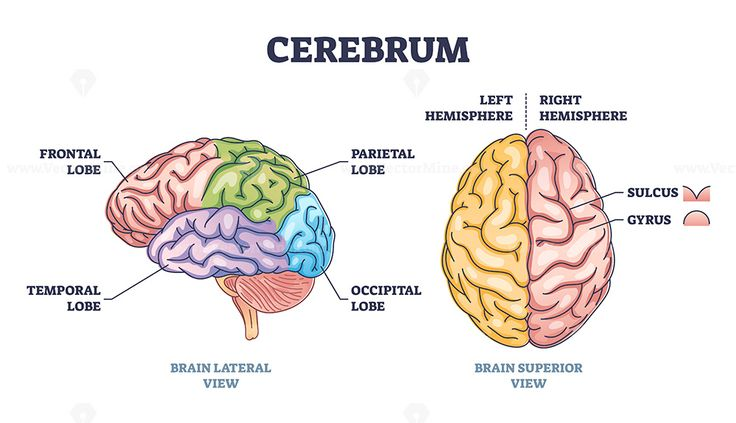
\includegraphics[width=0.7\textwidth]{Images/Chapter0/cerebrum.jpg}
  \caption{Cerebrum brain structure from lateral and superior view outline diagram.\cite{freudenrich2013visualizing}.}
  \label{fig:cerebrum}
\end{figure}

Each hemisphere contains four lobes—frontal, parietal, occipital, and temporal—with distinct functions (Figure~\ref{fig:cerebrum}).



\paragraph{Frontal lobes}
\begin{itemize}
  \item Speech, language, reasoning, decision-making, personality, judgment, and voluntary movements.
  \item Right frontal lobe controls left-side movements; left frontal lobe controls right-side movements.
\end{itemize}

\paragraph{Parietal lobes}
\begin{itemize}
  \item Reading, spatial and visual perception, touch, pain, and temperature sensation.
  \item Right parietal lobe mediates left-side sensitivity; left parietal lobe mediates right-side sensitivity.
\end{itemize}

\paragraph{Occipital lobes}
\begin{itemize}
  \item Visual processing (color, light, movement).
\end{itemize}

\paragraph{Temporal lobes}
\begin{itemize}
  \item Language comprehension, memory, and emotion processing.
  \item Sequencing and organization.
\end{itemize}

\subsubsection{Cerebellum}
The cerebellum lies below the cerebrum and accounts for about 11\% of brain volume. It coordinates reflexes, movement, balance, and posture.

\subsubsection{Brainstem}
The brainstem connects the cerebrum and cerebellum to the spinal cord and controls vital functions such as eye movements, breathing, blood pressure, and heart rate.

\subsubsection{Diencephalon}
Surrounded by the cerebral hemispheres, the diencephalon coordinates motor functions, maintains consciousness, regulates autonomic functions (eating, thirst, temperature, circadian rhythm) and interacts with both brain and cerebellum \cite{ref4}.
\subsection{Microscopic Description}
From a microscopic point of view, the nervous tissue consists of nerve
cells (neurons) and glial cells (support and protective cells) that derive
from the ectoderm. Vessels and meninges do not belong to the nervous
tissue and are derived from the mesoderm.
The neuron is the cell that constitutes the functional unit of the
neuroaxis. Neurons are 10 to 50 times more numerous than glial cells.
The human nervous system comprises about 100 billion neurons. Neurons
transmit a signal or what we call nerve impulses \cite{ref3}.

\section{Brain Tissue}
Accurate segmentation of brain tissues in MRI is critical for diagnosis and treatment planning. Anatomical structures can be divided into hemispheres and lobes, but for imaging, we often classify voxels as gray matter, white matter, or cerebrospinal fluid \cite{ref1}.

\subsection{Gray Matter}
Gray matter contains neuronal cell bodies (soma), axon tracts, glial cells, capillary blood vessels, and neuropil (dendrites, unmyelinated axons, glia) \cite{ref5}.

\subsection{White Matter}
White matter consists primarily of myelinated axons (tracts), oligodendrocytes, and astrocytes, forming the brain’s long-range connections \cite{ref5}.

\subsection{Cerebrospinal Fluid}
Cerebrospinal fluid (CSF) cushions the brain and spinal cord, removes metabolic waste, and maintains proper central nervous system function \cite{ref6}.

\begin{figure}[ht]
  \centering
  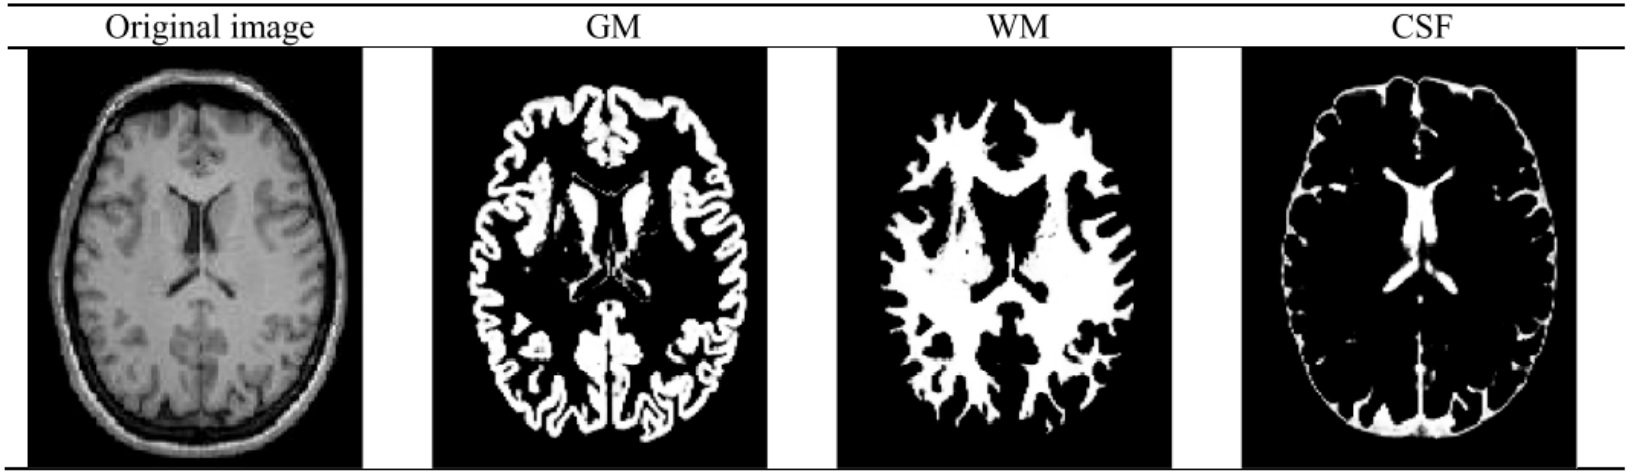
\includegraphics[width=0.7\textwidth]{Images/Chapter0/parts.png}
  \caption{Segmentation of a brain MRI into gray matter (GM), white matter (WM), and CSF by Statistical Parametric Mapping (SPM) \cite{ref7}.}
  \label{fig:spm-segmentation}
\end{figure}

\section{Classification of Brain Tumors}
\subsection{Benign Brain Tumors}
Benign brain tumors are made up of a group of cells, and their growth
10is slow, because these tumors originate from non-neuronal brain cells called
astrocytes, and they differ in the division and growth stages from normal
cells, and in microscopic analysis they do not have the same appearance
as cancer microscopically, because of their growth and their unique spread
from cancer cells. In most cases, they are benign, because they do not
invade surrounding tissues, but in turn, there are conditions that lead to
the same risk of malignant cancer cells, if these cells are forced into sensitive
areas of the brain, which in turn adversely affect vital functions.

\subsection{Premalignant Brain Tumors}
Premalignant tissues are not yet cancerous but have the potential to become malignant.

\subsection{Malignant Brain Tumors}
They are classified as ”cancerous”, defining certain primary tumors
as well as all metastatic brain lesions. They consist of cells that divide
relatively quickly. These tumors grow rapidly and can invade and damage
important brain structures. They can be treated with surgery, radiotherapy, chemotherapy or a combination of these \cite{ref8}.

\section{Signs and Symptoms Associated with Brain Tumors}
Symptoms depend on tumor location, patient age, and growth rate, and include focal deficits (motor, seizure, visual, speech) and generalized signs (headache, nausea, dizziness, sleep disturbances) \cite{ref9}.

\section{Diagnosis of Brain Tumors}
\subsection{Physical Examination}
Neurological exam assesses functions controlled by each brain lobe (memory, language, sensation) to localize lesions.

\subsection{Complementary Examination}
May include lumbar puncture to analyze CSF for tumor cells.

\subsection{Brain Biopsy}
Surgical removal of tissue sample for histopathology, with risks of bleeding and infection.

\subsection{Medical Imaging}
Techniques include MRI and CT; MRI is preferred for its soft-tissue contrast.

\subsubsection{Magnetic Resonance Imaging (MRI)}
MRI produces high-resolution anatomical images based on nuclear magnetic resonance. Since its first demonstration in 1973 by Lauterbur and Damadian, MRI has evolved to 2D, 3D, and even 4D acquisitions \cite{ref10}.

\subsubsection{Main Components of MRI}
An MRI system comprises:
\begin{itemize}
  \item The main magnet (B$_0$) in Tesla.
  \item Gradient coils (X, Y, Z) for spatial encoding.
  \item Radiofrequency antennas for transmission and reception.
  \item A computer for pulse sequencing, data acquisition, Fourier reconstruction, and image storage \cite{ref11,ref12}.
\end{itemize}

\subsubsection{Acquisition of MRI Images}
Adjustable parameters TR (repetition time) and TE (echo time) define T1-, T2-, or proton-density weightings. Contrast agents (e.g., gadolinium) enhance specific tissue signals \cite{ref11}.

\begin{figure}[ht]
  \centering
  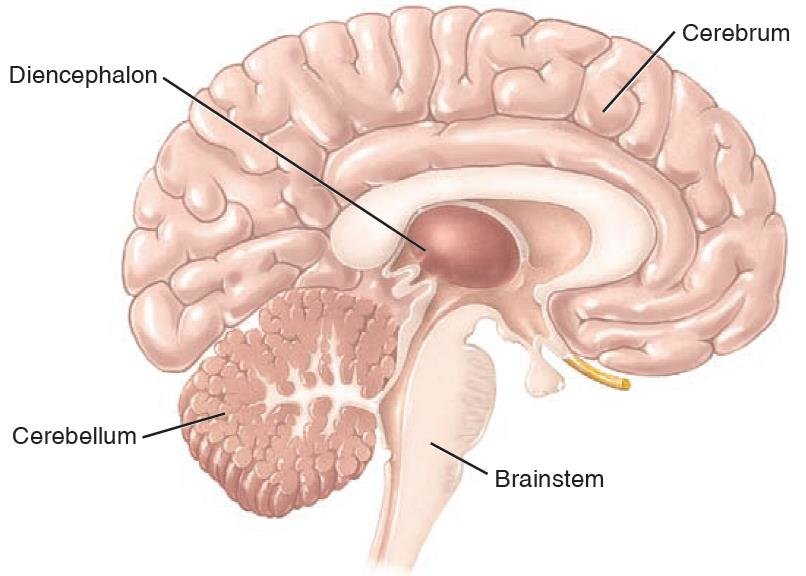
\includegraphics[width=0.7\textwidth]{./Images/Chapter0/brain.jpg}
  \caption{MRI acquisition: (a) T1-weighted; (b) T2-weighted \cite{ref11}.}
  \label{fig:mri-acquisition}
\end{figure}

